\subsection{Milestones}
From a project management perspective, the team will be utilizing Agile to get quick turn arounds on small deliverables. Choosing to use agile, the team will also be using Jira to track progress and add reports throughout the process. A high-level of the goals by semester can be found below.
\subsubsection{Fall}
\begin{itemize}
    \item Select components for each subsystem
    \begin{itemize}
        \item Document selection reasoning
        \item Order to ensure on-time delivery
    \end{itemize}
    \item Model physical bed
    \item Build physical bed
    \item Understand how subsystems will integrate:
    \begin{itemize}
        \item Communication protocols (REST, I2C, SPI, DSP, etc)
        \item Power requirements
    \end{itemize}
    \item UI for Web subsystem
\end{itemize}
\subsubsection{Spring}
\begin{itemize}
    \item Test subsystems in isolation
    \item Start integrating subsystems
    \item Control scheme for moving solar panels with sun and to provide shade
    \item Web API complete
    \item MCU coding complete
    \item Stretch goals
\end{itemize}

\subsection{Progress}

\subsubsection{Senior Design I}
\begin{figure}[H]
    \caption{Cumulative Flow Diagram from Jira}
    \centering
    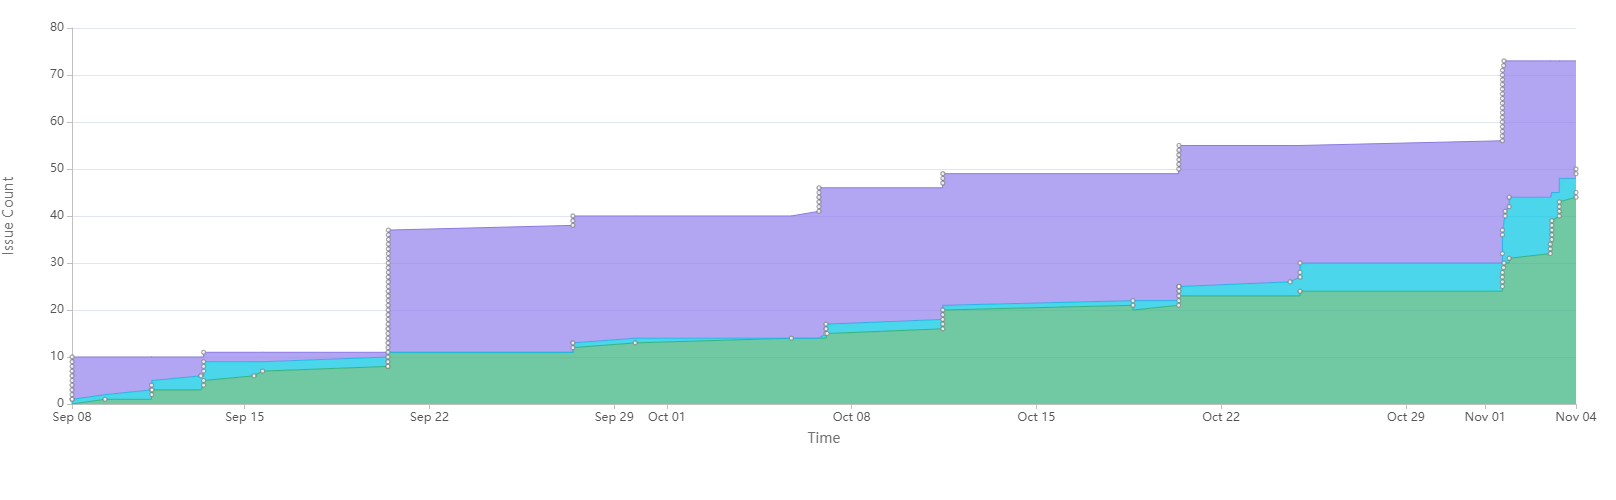
\includegraphics[width=\textwidth]{images/Cumulative flow diagram.png}
    \label{fig:cumulativeflow}
\end{figure}
In Figure \ref{fig:cumulativeflow}: purple designates tasks that are marked unfinished in the the backlog and current sprint, blue represents in progress tasks, and green represents finished tasks.

Throughout Senior Design I we have been gathering research and have started laying out the design of our garden bed and have completed the majority of our part selection. The Figure in \ref{fig:cumulativeflow} may be a little misleading at this point because we have not refined our backlog to fully encapsulate meaningful tasks instead breaking it down into larger subsystem requirement-esque tasks.

